\documentclass[11pt]{article}

\usepackage[margin=1in]{geometry}
\usepackage[T1]{fontenc}
\usepackage{lmodern}
\usepackage{microtype}
\usepackage{amsmath}
\usepackage{booktabs}
\usepackage{tabularx}
\usepackage{graphicx}
\usepackage{enumitem}
\usepackage[dvipsnames]{xcolor}
\usepackage{caption}
\usepackage[round,authoryear]{natbib}
\definecolor{linkblue}{HTML}{1A5FB4}
\usepackage[colorlinks=true,citecolor=linkblue,linkcolor=linkblue,urlcolor=linkblue]{hyperref}

\setlength{\parskip}{0.45em}
\setlength{\parindent}{0pt}
\setlist{itemsep=0.25em,topsep=0.3em}
\captionsetup{font=small,labelfont=bf}
\newcolumntype{L}{>{\raggedright\arraybackslash}X}

\title{\textbf{State Shock Ledger: Methods Note}\\[0.3em]\large Prototype version 0}
\author{Samson M'boueke}
\date{October 8, 2026}

\begin{document}
\maketitle

\begin{abstract}
\noindent The State Shock Ledger measures how movements in world commodity prices change
income across the fifty U.S.\ states and the District of Columbia. For each state and
commodity it records the state's net position, production minus consumption, and values
the change in the world price against it. The result is reported in dollars and as a share
of state GDP, monthly from January 2000, daily for energy, and forward over the horizon of
the Energy Information Administration's price outlook. This note documents the definitions,
data, and limitations of version 0. Every figure in the prototype is rebuilt from public
data by the accompanying code.
\end{abstract}

\section{Measure}

For state $s$, commodity $c$ and month $t$, the windfall is
\begin{equation}
  W_{s,c,t} \;=\; N_{s,c,Y(t)} \times \bigl(p_{c,t} - p_{c,t-12}\bigr),
  \label{eq:windfall}
\end{equation}
where $p_{c,t}$ is the world benchmark price and $N_{s,c,Y}$ is the state's net position in
the commodity for the calendar year $Y$ that contains month $t$. $W$ is an annualized dollar
flow: the change in the value of one year of the state's net position caused by the price
change over the previous twelve months. The state total sums over commodities, and the
share of GDP divides by current-dollar state GDP for year $Y$, carrying the latest year
published by the Bureau of Economic Analysis forward.

The construction adapts the commodity terms-of-trade database of \citet{gruss2019}, which
weights world commodity prices by country net exports to proxy windfall income gains and
losses, from countries to U.S.\ states.

\paragraph{Net positions.} Positions are the average of the three calendar years before
$Y$, that is, years $Y-3$ to $Y-1$. Lagged weights keep the measure driven by prices rather
than by the state's own output response. Beyond the last year of source data, the latest
three available years are used. Table~\ref{tab:positions} lists the definitions.

\begin{table}[ht]
\centering
\small
\caption{Net positions and benchmark prices, version 0}
\label{tab:positions}
\begin{tabularx}{\textwidth}{@{}>{\raggedright\arraybackslash}p{2.3cm} L
  >{\raggedright\arraybackslash}p{1.7cm} >{\raggedright\arraybackslash}p{2.5cm}@{}}
\toprule
Commodity & Net position & Unit & Benchmark price \\
\midrule
Crude oil & Crude production minus crude-priced petroleum use: total petroleum
  consumption less hydrocarbon gas liquids, petroleum coke and refinery still gas
  (SEDS codes PAPRP, PATCP, HLTCP, PCTCP, SGICP) & barrels & WTI \\
\addlinespace
Natural gas & Marketed production minus total consumption (SEDS codes NGMPB, NGTCB)
  & MMBtu & Henry Hub \\
\addlinespace
Corn, soybeans, wheat, cattle & Farm cash receipts divided by the mean world price over
  the same years; producer side only & world price unit & Maize; soybeans; wheat (US HRW);
  beef \\
\bottomrule
\end{tabularx}
\end{table}

\paragraph{Why the petroleum exclusions.} Hydrocarbon gas liquids such as ethane and
propane are mostly petrochemical feedstocks priced off natural gas and petrochemical
markets, not crude oil. Petroleum coke and still gas are refinery-internal fuels whose cost
is passed to buyers of refined products, often in other states. Without the exclusions,
refining and petrochemical states such as Louisiana and Texas appear to bear costs that are
in fact passed on. In 2024 the exclusions remove 1.68 billion of the 7.49 billion barrels of
U.S.\ petroleum use (gas liquids 1.37 billion, still gas 0.23 billion, petroleum coke 0.08
billion).

\paragraph{Consumer pass-through for oil.} Consumers are assumed to pay roughly the crude
price change per barrel of refined product. Refining margins, taxes and regional price
differences are ignored in version 0.

\section{Views}

\begin{description}[leftmargin=1.6em,style=nextline]
  \item[History] Monthly World Bank prices and the twelve-month change in
  equation~\eqref{eq:windfall}, from January 2000.
  \item[Latest] Energy uses the latest EIA daily spot price against the mean of the same
  seven-day window one year earlier. Agriculture uses the latest World Bank month.
  \item[Outlook] The latest EIA Short-Term Energy Outlook monthly path for WTI and Henry
  Hub, against the mean of the last twelve months of prices, valued at current positions.
  \item[Scenario] User-chosen oil and gas prices against the same twelve-month base.
\end{description}

Figure~\ref{fig:states} shows the history for four states with different commodity
profiles. North Dakota's position is dominated by crude oil, Texas is long in both oil and
gas but is also a large consumer, Iowa's swings come from corn and soybeans, and California
is a net consumer of energy.

\begin{figure}[ht]
\centering
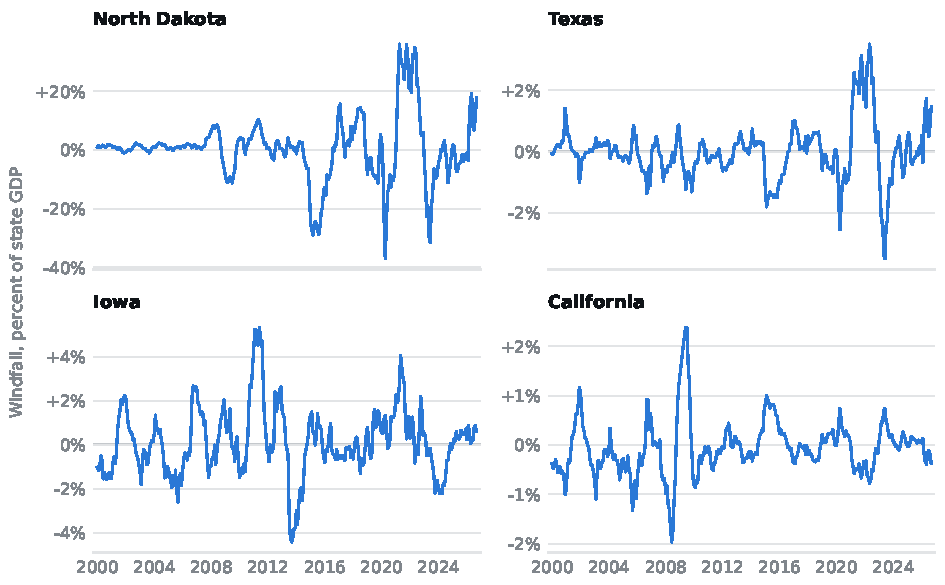
\includegraphics[width=\textwidth]{fig_states.pdf}
\caption{Monthly commodity windfall, all covered commodities, percent of state GDP,
January 2000 to September 2026. Vertical scales differ across panels. Prototype figures,
gross values at benchmark prices; see Section~\ref{sec:limits}.}
\label{fig:states}
\end{figure}

\section{Interpretation and limitations}
\label{sec:limits}

\begin{enumerate}[leftmargin=1.4em]
  \item \textbf{Gross value, not income.} $W$ values production and use at benchmark
  prices. It is an upper bound on the change in income accruing in the state, because part
  of the windfall goes to owners, royalty holders and shareholders elsewhere
  \citep{feyrer2017}, and because wellhead prices differ from WTI and Henry Hub. Rocky
  Mountain gas trades at a discount to Henry Hub, which inflates gas-state swings such as
  Wyoming's in 2008 and 2009.
  \item \textbf{Agriculture is producer side only.} The farm share of retail food spending
  is small and pass-through is slow, so the consumer side is second order at monthly
  frequency. Feed use by livestock states is not netted out. Both are planned.
  \item \textbf{Federal offshore production} (SEDS areas X3 and X5) belongs to no state and
  is reported separately. Its windfall accrues to producers and, through royalties, to the
  federal government.
  \item \textbf{Coal, copper and potash} are not in version 0. Coal needs a U.S.\ price
  series, because domestic coal is sold under contracts. Copper and potash need state
  production data, which the U.S.\ Geological Survey often withholds for confidentiality.
  \item \textbf{Futures.} The EIA stopped publishing free NYMEX futures prices after April
  5, 2024, so the version 0 outlook uses the EIA's own forecast. Licensed futures and options
  data would allow market-implied outlooks with uncertainty bands.
\end{enumerate}

\section{Validation plan}

The Ledger is useful to the extent that windfalls predict state outcomes. A companion
working paper will estimate local projections \citep{jorda2005} of state employment,
personal income, prices and tax revenue on the windfall, with state and time fixed effects
over 2000 to 2025. It will report responses at horizons of zero to twenty-four months and
test whether the net measure outperforms production-only and consumption-only exposures.
The estimated responses will then supply the dashboard's projected consequences for each
state.

\section{Data and reproduction}

All inputs are public and require no registration: the EIA State Energy Data System, daily
spot prices and Short-Term Energy Outlook; the USDA Economic Research Service Farm Income
and Wealth Statistics; the World Bank Commodity Price Data; and the Bureau of Economic
Analysis GDP by state. Three scripts download the inputs, build the ledger, and package the
dashboard. A checksum manifest records the exact input files used, so that a provider's
revision of a series is detectable.

\begin{thebibliography}{9}
\setlength{\itemsep}{0.3em}
\bibitem[Feyrer et~al.(2017)Feyrer, Mansur, and Sacerdote]{feyrer2017}
Feyrer, J., E.~T. Mansur, and B.~Sacerdote (2017). Geographic dispersion of economic
shocks: Evidence from the fracking revolution. \emph{American Economic Review} 107(4),
1313--1334.

\bibitem[Gruss and Kebhaj(2019)]{gruss2019}
Gruss, B. and S.~Kebhaj (2019). Commodity terms of trade: A new database. IMF Working
Paper WP/19/21, International Monetary Fund.

\bibitem[Jord{\`a}(2005)]{jorda2005}
Jord{\`a}, {\`O}. (2005). Estimation and inference of impulse responses by local
projections. \emph{American Economic Review} 95(1), 161--182.
\end{thebibliography}

\end{document}
